\usepackage[spanish]{babel}
\usepackage{circuitikz}[american]
\usepackage{amsmath,eso-pic}
\usepackage{pgfplots}
\usepackage{sectsty}
\usepackage{newtxtext,newtxmath,subfiles}
\usepackage[]{toolsgf}
\usepackage{titlesec}

\newcommand\BackgroundPic{%
  \put(-90,0){%
    \parbox[b][\paperheight]{\paperwidth}{%
      \vfill
      \centering
      % Aquí especificamos tu ruta: /images/background.png
      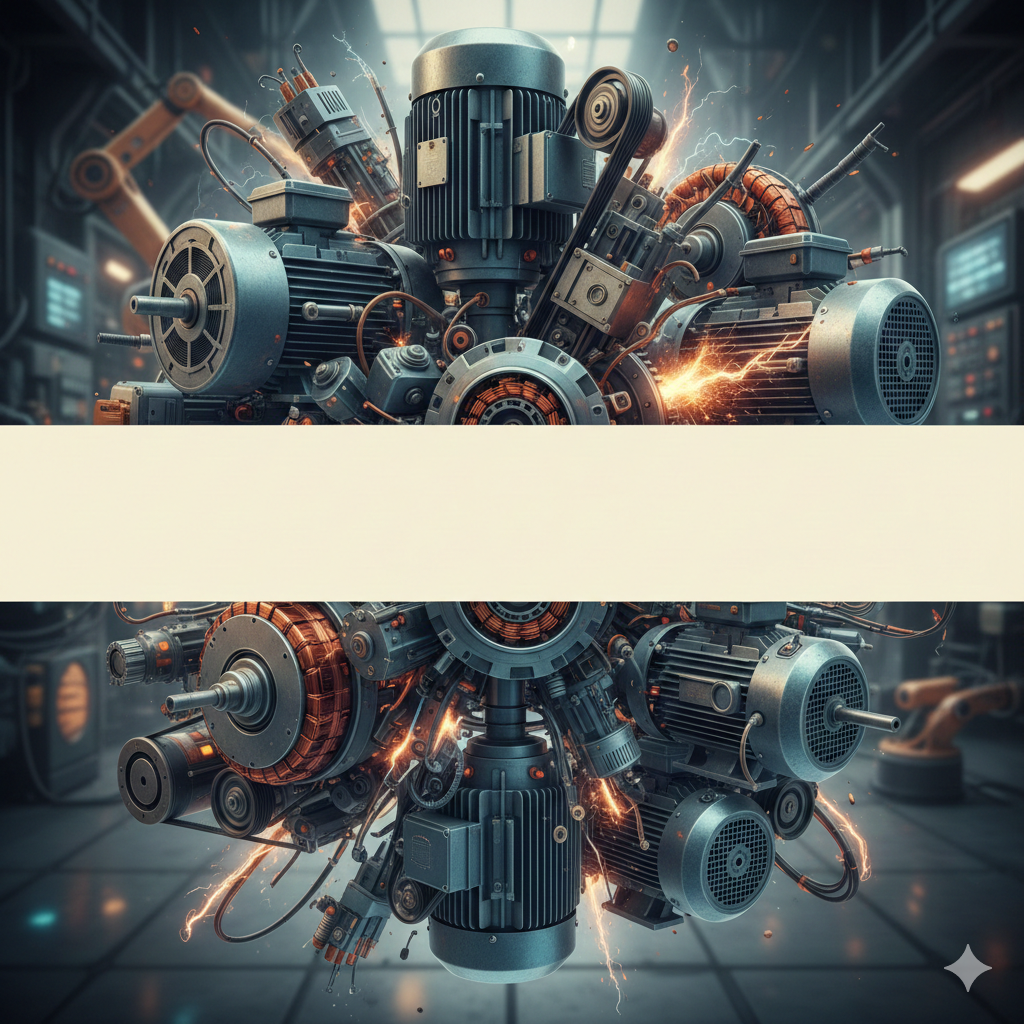
\includegraphics[height=\paperheight,keepaspectratio=true]{images/background.png}%
      \vfill
    }
  }
}
\allsectionsfont{\sffamily}
\pgfplotsset{compat=1.7}

\newcommand{\materia}{MÁQUINAS  ELÉCTRICAS II}
\newcommand{\TP}{}
\newcommand{\logo}{images/4124}
\newcommand{\email}{gustavo@merin.edu.ar}
\newcommand{\classroomcode}{6sgmgfkt}
\newcommand{\urlqr}{https://www.merin.edu.ar/}

\title{\vspace{3.5cm}\Huge Guía de Trabajos Prácticos\\\textbf{\materia}}
\author{Ferreyra G.}
\date{Año: 2026}

\sectionfont{\sffamily}
\subsectionfont{\sffamily}
\titleformat{\chapter}{\sffamily\huge}{\textbf{Trabajo Práctico
N$^\circ$:\thechapter}}{20pt}{\centering}
